\subsection{Decision Range (DR) and Abort/Skate/Banzai}

\subsubsection*{Simple Definitions}

\begin{itemize}
  \item Abort: Emergency egress

  \item Skate: Planned egress

  \item Decision Range: The range NLT you can perform a notch and assess whilst
    being able to Abort

  \item Banzai: Head into the merge (press)

  \item F-Pole: The distance from launcher to target if the shot were now

  \item MAR: Minimum Abort Range; the closest Range at which you can safely
    turn from the fight and run from a specific enemy missile.

\end{itemize}

\subsubsection*{General}

Once in the Crank, the Flight has to monitor several items:

\begin{itemize}
  \item RWR - Enemy Spikes (Plane and Missile)
  \item Defending via chaff
  \item Gimbals and missile support
  \item Pitbull and Timeout
  \item Relative altitude differences (avoiding being notched)
  \item Enemy defending (opportunities to Banzai)
  \item Range, especially Minimum Abort Range
\end{itemize}

Culminating in the choice to Banzai, Skate or Abort.

This phase is quite complex and of the hardest workload.

\sidebyside{0.5}{%
  Thus far the flight has given good total energy package to the missile shot,
  at the bandit, at the correct range, then increased the Bandit's F-pole to
  lengthen the travel distance of a return shot. At the point where there are
  missiles in the air and possibly returned shots, the flight leader has to
  concern themselves with what to do next.
}{
  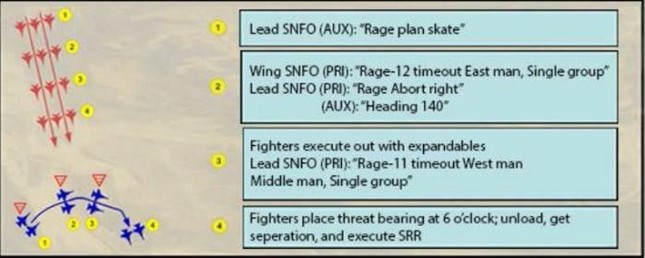
\includegraphics[width=\textwidth,align=t]{bvr/decision}
}

The safest goal for a long shot is to Skate out and exit the fight with an open
mind to recommit, once the missile is properly under its own guidance.
\textbf{The Tomcat should never ordinarily choose to merge whilst other options
exist to succeed in the Mission}. The flight can still monitor the shot using
the count down timer. There is no Pitbull timer for when the AIM-54 goes
active, however it can be interpreted from the timer and range. At 15nm Pitbull
range, napkin maths gives us a bit more than half of the original timer count.
So, with a 90 second shot, we can call Pitbull at 40 seconds to go. We should
note: DCS is not as fussy yet as the missile code is simplified

At Pitbull the Pilot needs to put the enemy on the 3-9 line and notch. At this
point the crew are looking for Spikes/Nails, performing chaffing, observing the
relative aspect and altitude of the Bandit and its range for determining the
Minimum Abort Range (MAR). Knowing the Bandit's MAR is a matter of Briefing and
experience.

Should the Bandit drop their spike and appear defensive in aspect or altitude
change, the choice to Press or "Banzai" could be made

\boxed{%
  Note: Most of this is advanced and kept for CT and A-A TTP 1 and 2. For now,
  all that is required to know is that there are three choices and three
  possible calls on Pri; to "Banzai", "Skate" or to "Abort".
}

\subsubsection*{Example}


\textbf{FL RIO (Pri):} "1, Pitbull!"\\
\textbf{WM RIO (Pri):} "2, Pitbull!"\\
\textbf{FL RIO (Pri):} "1 Timeout and Naked, Spectre Banzai!"\\

\textbf{Or}

\textbf{FL RIO (Pri):} "1, Pitbull!"\\
\textbf{FL RIO (Pri):} "1, Spiked"\\
\textbf{FL RIO (Pri):} "Spectre 1, Abort 180"\\

\boxed{%
  Both RIO's will call out Spikes on RWR and transitions to Naked or any change
  thereof. They will also monitor their own shot and report both Pitbull and
  Timeout if possible. At Pitbull they release the gimbal lock and put any
  threat on the 3-9 before making a decision on whether to Abort or Banzai.
}
